%!TEX root = main.tex


\section{Causal Bayesian Networks}\label{sec:CBN}

So, what is a causal Bayesian network? According to \citet{pearl_causality:_2009}, a probability model $\prob{P}$, a directed acyclic graph $\mathcal{G}$ whose nodes are identified with some collection of variables $\{\text{Pa}(\RV{X}),\RV{X},\RV{Y}\}$, and a collection of interventional probability models $\{\prob{P}_{\RV{X}=a}|a\in X_i\}$ such that the interventional probability models all obey the truncated factorisation condition with respect to $\mathcal{G}$.

The truncated factorisation condition holds that
\begin{align}
    \prob{P}_{\RV{X}=a}^{\text{Pa}(\RV{X})\RV{X}\RV{Y}}(a,b,c) &= \prob{P}^{\text{Pa}(\RV{X})}(a)\prob{P}^{\RV{Y}|\text{Pa}(\RV{X})}(c|a)\llbracket x=a \rrbracket
\end{align}

Let's slow down for a second. What are these variables $\{\text{Pa}(\RV{X}),\RV{X},\RV{Y}\}$, and what do we mean they are distributed according to $\prob{P}$? It means that we have a sequence of variables $\RV{V}_A:=(\text{Pa}(\RV{X}_i),\RV{X}_i,\RV{Y}_i)_{i\in A}$ modelled by $\prob{P}^{\RV{V}_A|\RV{H}}$ such that the triples $(\text{Pa}(\RV{X}_i),\RV{X}_i,\RV{Y}_i)$ are mutually independent and identically distributed conditonal on $\RV{H}$. For each $h\in H$ we have a probability measure $\prob{P}^{\RV{V}_i|\RV{H}}(\cdot|h)$ (for any $i$) that uniquely defines $\prob{P}^{\RV{V}_A|\RV{H}}(\cdot|h)$. 



Let's be honest here, this ``collection of interventional distributions'' is really a model. We have a Markov kernel $\kernel{Q}:=a\mapsto \prob{P}_{\RV{X}=a}$, and the indices are clearly going to designate the codomain as a model of $(\text{Pa}(\RV{X}),\RV{X},\RV{Y})$, and the domain is proposed value of $\RV{X}$. So we have a model $\model{Q}^{\text{Pa}(\RV{X})\RV{X}\RV{Y}|\RV{X}}$.  which is well defined at least if $\{\text{Pa}(\RV{X}),\RV{X},\RV{Y}\}$ are mutually variationally independent. Now, how does $\model{Q}^{\cdot|\RV{X}}$ relate to $\prob{P}$? Let's draw them out:



In the presentation of \citet{pearl_causality:_2009}, a Causal Bayesian Network posits an observational probability distribution such as $P(X,Y)$, and a set of interventional distributions, for example $\{\prob{P}_h(X,Y|do(X=x))\}_{x\in X,h\in H}$. Here we use notation similar to typical notation used for Causal Bayesian Networks and don't intend for these to necessarily be elements of any modelling context. For simplicity, we will consider a Causal Bayesian Network with only hard interventions on a single variable, e.g. interventions only of the form $do(\RV{X}=x)$.

First we will offer some commentary



We can consider this an instance of a see-do model. To do so consistently within a modelling context $\mathscr{M}$, we need to distinguish observation and intervention variables - let the former retain the labels $\RV{X},\RV{Y}$ and call the latter $\RV{X}',\RV{Y}'$. Let $D=\{do(\RV{X}=x)\}_{x\in X}$. Then a Causal Bayesian Network can be considered a see-do model $\model{T}[\RV{XYX'Y'}|\RV{HD}]$ by identifying $\model{T}[\RV{XY}|\RV{H}]_h := \prob{P}_h(X,Y)$ and $\model{T}[\RV{X'Y'}|\RV{HD}]_{h,do(\RV{X}=x)}:={P}_h(X,Y|do(X=x))$.

\todo[inline]{We need to rename the consequence variables because otherwise we would have $\model{T}[\RV{XYXY}|\RV{HD}]$ and the two $\RV{X}$'s and the two $\RV{Y}$'s would be deterministically equal by the ``identical labels'' rule}

We can say a bit more about Causal Bayesian Networks. Suppose we have the network
\begin{align*}
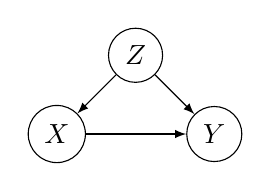
\begin{tikzpicture}
    \path (0,0) node[draw,circle] (X) {$\RV{X}$}
    ++ (1,1) node[draw,circle] (Z) {$\RV{Z}$}
    ++ (1,-1) node[draw, circle] (Y) {$\RV{Y}$};
    \draw[-latex] (X)--(Y);
    \draw[-latex] (Z) -- (Y);
    \draw[-latex] (Z) -- (X);
\end{tikzpicture}
\end{align*}

Then, letting $\model{T}[\RV{XYZ}|\RV{H}]$ be the observational ``see'' model and $\model{T}[\RV{X'Y'Z'}|\RV{HD}]$ be the interventional ``do'' model with $D$ the set of interventions $\{do(\RV{X}=x)\}_{x\in X}$ where we write $x:=do(\RV{X}=x)$ for short, then we know by the backdoor adjustment rule that $\model{T}[\RV{X'Y'Z'}|\RV{HD}]_{hx}^{x'yz} \overset{krn}{=} \model{T}[\RV{Z}|\RV{H}]_h^z \delta[x]^{x'} \model{T}[\RV{Y}|\RV{XZH}]_{hx'z}^y$. 

Let $\model{U}[\RV{ZY}|\RV{XH}] = \model{T}[\RV{Z}|\RV{H}]\rightrightarrows \model{T}[\RV{Y}|\RV{XZH}]$, call $\model{T}[\RV{X}|\RV{H}]$ the ``observational strategy'' and $\model{D}_x[\RV{X}|\RV{D}]_x^{x'} \overset{krn}{=} \delta[x]^{x'}$ the interventional strategies for all $x\in X$. Then we have

\begin{align}
    \model{T}[\RV{XYZ}|\RV{H}] &= \model{U}[\RV{Z}|\RV{H}]\rightrightarrows \model{T}[\RV{X}|\RV{H}] \rightrightarrows \model{U}[\RV{Y}|\RV{XHZ}]\\
    \model{T}[\RV{X'Y'Z'}|\RV{HD}] &\overset{krn}{=} \model{U}[\RV{Z}|\RV{H}]\rightrightarrows \model{D}[\RV{X}|\RV{D}] \rightrightarrows \model{U}[\RV{Y}|\RV{XHZ}]
\end{align}
So this simple example of a Causal Bayesian network is a ``nested comb'' where the outer comb $\model{T}[\RV{XYZX'Y'Z'}|\RV{HD}]$ is the ``see'' and ``do'' models, which are themselves generated by the inner comb $\model{U}[\RV{ZY}|\RV{XH}]$ with different choices $ \model{T}[\RV{X}|\RV{H}]$ and $\model{D}[\RV{X}|\RV{D}]$ for the insert.

This is a simple example, but \citet{jacobs_causal_2019} has used an ``inner comb'' representation of a general class of Causal Bayesian Networks to prove a sufficient identification condition which is itself slightly more general than the identification condition given by \citet{tian2002general}.